%--------- プリアンブル ---------%
\documentclass[dvipdfmx, 12pt]{beamer}
\usepackage{bxdpx-beamer}                         % dvipdfmx には必要
\usepackage{pxjahyper}                            % しおりの文字化けを防ぐ
\usepackage{minijs}                               % フォントメトリックをまともに

% パッケージ
\usepackage{otf, ascmac, graphicx, multicol, tikz, listings, xytree}
\renewcommand{\kanjifamilydefault}{\gtdefault}


\usetikzlibrary{arrows.meta, shapes.callouts}

\tikzset{callout/.style={rectangle callout, rounded corners, white, fill=red!75, minimum height=30pt}}
\tikzset{probrem/.style={rectangle, white, fill=red!75, text centered, font=\huge, minimum width=24zw}}

\tikzset{block/.style={rectangle, rounded corners, draw, text centered, minimum height=20pt}}
\tikzset{progress/.style={block, fill=cyan!12}}
\tikzset{progress10/.style={progress, minimum width=10zw}}
\tikzset{progress20/.style={progress, minimum width=20zw}}
\tikzset{success/.style={block, fill=magenta!12, minimum width=10zw}}
\tikzset{failure/.style={block, red, fill=red!12}}

\lstset{
    basicstyle=\ttfamily\footnotesize,
    commentstyle=\color[rgb]{0.0,0.6,0.0},
    backgroundcolor=\color[rgb]{0.95,0.95,0.92},
    columns=[l]{fullflexible},
    frame=tlBR,
    framesep=5pt,
    lineskip=-0.3ex,
    breaklines=true,
    breakatwhitespace=false,
    keepspaces=true,
    showspaces=false,
    showstringspaces=false,
    showtabs=false
}

\colorlet{number}{green!60!black}
\definecolor{bracket}{RGB}{20,100,175}

\lstdefinelanguage{json}{
    keywords={null, true, false},
    keywordstyle=\color{blue!60!black},
    literate=
       *{0}{{{\color{number}0}}}{1}
        {1}{{{\color{number}1}}}{1}
        {2}{{{\color{number}2}}}{1}
        {3}{{{\color{number}3}}}{1}
        {4}{{{\color{number}4}}}{1}
        {5}{{{\color{number}5}}}{1}
        {6}{{{\color{number}6}}}{1}
        {7}{{{\color{number}7}}}{1}
        {8}{{{\color{number}8}}}{1}
        {9}{{{\color{number}9}}}{1}
        {\{}{{{\color{bracket}{\{}}}}{1}
        {\}}{{{\color{bracket}{\}}}}}{1}
        {[}{{{\color{bracket}{[}}}}{1}
        {]}{{{\color{bracket}{]}}}}{1},
    numbers=left,
    numberstyle=\scriptsize,
    firstnumber=1,
    stepnumber=1,
    numbersep=9pt
}

\hypersetup{
    setpagesize=false,
    bookmarksnumbered=true,
    bookmarksopen=true,
    colorlinks=true,
    linkcolor=blue!75,
    urlcolor=teal!60
}


% 設定情報
\usetheme[]{metropolis}
\usefonttheme{professionalfonts}

\setbeamercolor{normal text}{bg=white}
\setbeamercolor{enumerate item}{fg=blue!75}
\setbeamercolor{description item}{fg=blue!75}

\setbeamertemplate{caption}{\raggedright\insertcaption\par}
\setbeamertemplate{navigation symbols}{}

\setbeamercolor{footline}{fg=red!75}
\setbeamertemplate{footline}[page number]
\setbeamerfont{footline}{series=\bfseries}

\AtBeginSection[]{
    \begin{frame}{目次}
        \tableofcontents[currentsection]
    \end{frame}
}


% 属性情報
\title{Dockerfileの開発を支援する\\インタラクティブツールの提案}
\author{稲田 司}
\institute{\small 鵜林・亀井研究室}
\date{2023/02/17}


% 変数定義
\newlength{\mytotalwidth}
\newlength{\mycolumnwidth}
\mytotalwidth=\dimexpr\linewidth-5mm
\mycolumnwidth=\dimexpr\mytotalwidth-5mm




%--------- スライド ---------%
\begin{document}


\frame{\maketitle}

\begin{frame}{目次}
    \tableofcontents
\end{frame}


\section{導入}

\begin{frame}{Dockerとは何か?}
    ソフトウェアの実行に必要なものすべてを\textcolor{red!75}{パッケージ化}し,
    それらを\textcolor{red!75}{プロセスレベル}で分離された空間で実行する技術.
    \vskip1.0zh

    % 仮想化技術としてのメリットもある
    \begin{itembox}[l]{ソフトウェア開発面でのメリット}
        \begin{itemize}
            \item ハードやOSの違いを意識せず,開発に専念できる.
            \item 既存の成果物を活用できる.
            \item アプリケーションのデプロイ・スケーリングが容易.
        \end{itemize}
    \end{itembox}
\end{frame}


\begin{frame}{Dockerfileとは何か?}
    Dockerにおいて,
    \begin{description}
        \item[イメージ] OSやアプリケーションのテンプレート
        \item[コンテナ] イメージを元に生成されるアプリケーション環境
    \end{description}

    Dockerfileは,イメージ構築を自動化する一連の命令群が記載されたテキストファイル.

    \begin{columns}[totalwidth=\mytotalwidth]
        \begin{column}[T]{0.05\mycolumnwidth}
        \end{column}
        \begin{column}[T]{0.25\mycolumnwidth}
            \begin{figure}
                \centering
                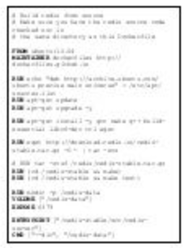
\includegraphics[height=60pt]{img/dockerfile.png}
                \caption{Dockerfile}
            \end{figure}
        \end{column}
        \begin{column}[T]{0.1\mycolumnwidth}
            \vskip2.0zh
            \centerline{build}
            \centerline{$\longrightarrow$}
        \end{column}
        \begin{column}[T]{0.3\mycolumnwidth}
            \begin{figure}
                \centering
                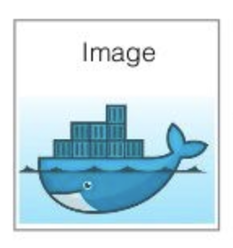
\includegraphics[height=60pt]{img/image.png}
                \caption{イメージ}
            \end{figure}
        \end{column}
        \begin{column}[T]{0.1\mycolumnwidth}
            \vskip1.0zh
            \centerline{run}
            \centerline{$\longrightarrow$}
            \centerline{\footnotesize (commit)}
            \centerline{$\dashleftarrow$}
        \end{column}
        \begin{column}[T]{0.3\mycolumnwidth}
            \begin{figure}
                \centering
                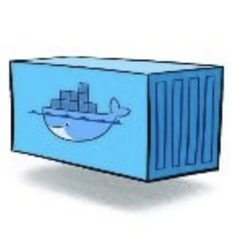
\includegraphics[height=60pt]{img/container.png}
                \caption{コンテナ}
            \end{figure}
        \end{column}
    \end{columns}
\end{frame}




\section{背景と目的}

\begin{frame}{イメージ・Dockerfileが抱える課題とその解決手法}
    \begin{multicols}{2}
        \begin{list}{}{\setlength{\itemsep}{1.0zh}}
            \setlength{\itemindent}{-3.0zw}
            \item ビルド時間の短縮
            \item イメージサイズの削減
            \item イメージ分析
            \item サイバー攻撃への対策
            \item 同一性の確認
            \item 再現性の確保
            \item イメージ開発の効率化
            \item 保守性の確保
        \columnbreak
        \setlength{\itemindent}{-4.6zw}
            \begin{onlyenv}<2->
                \item[→] キャッシュの利用,BuildKit
                \item[→] マルチステージビルド,DockerSlim
                \item[→] dive,dlayer
                \item[→] Distrolessイメージ,BuildKit
                \item[→] ハッシュによる確認,イメージ署名
                \item[→] ?
            \end{onlyenv}
            \begin{onlyenv}<2-3>
                \item[→] ?
                \item[→] ?
            \end{onlyenv}
            \begin{onlyenv}<4>
                \item[→] \textcolor{red!75}{インタラクティブツール}
                \item[→] \textcolor{red!75}{リファクタリングツール}
            \end{onlyenv}
        \end{list}
    \end{multicols}

    \begin{tikzpicture}[remember picture]
        \useasboundingbox (0.0, 0.0);
        \begin{scope}[shift={(current page.south west)}]
            \begin{tikzpicture}[remember picture, overlay]
                \begin{onlyenv}<3>
                    \node[callout, callout absolute pointer={(5.6, 2.2)}] at (8.8, 1.8) {本ツールで解決したい};
                    \node[callout, callout absolute pointer={(5.6, 1.2)}] at (8.8, 1.8) {本ツールで解決したい};
                \end{onlyenv}
            \end{tikzpicture}
        \end{scope}
    \end{tikzpicture}
\end{frame}




\section{本ツールの特長}

\begin{frame}{なぜ,イメージ開発の効率化が必要なのか?}
    下のギャップが,開発を非効率にしている.
    \begin{description}[labelwidth=6zw]
        \item[イメージ開発] Dockerfileを作成する必要がある.
        \item[動作確認] コンテナ内で行う必要がある.
    \end{description}

    \vskip1.0zh
    現状の動作確認の手法
    \begin{enumerate}
        \item 別で,同じベースイメージから起動したコンテナを使う.
        \item 開発途中のDockerfileから逐一生成するコンテナを使う.
    \end{enumerate}

    \vskip0.5zh
    どちらの手法も,\textcolor{red!75}{問題あり}.
\end{frame}


\begin{frame}{別で,同じベースイメージから起動したコンテナで\\動作確認をしながら,Dockerfileを開発する例}

\href{https://user-images.githubusercontent.com/103095414/209308363-14a95e02-4351-4036-a222-39e6a08a2982.mp4}{
    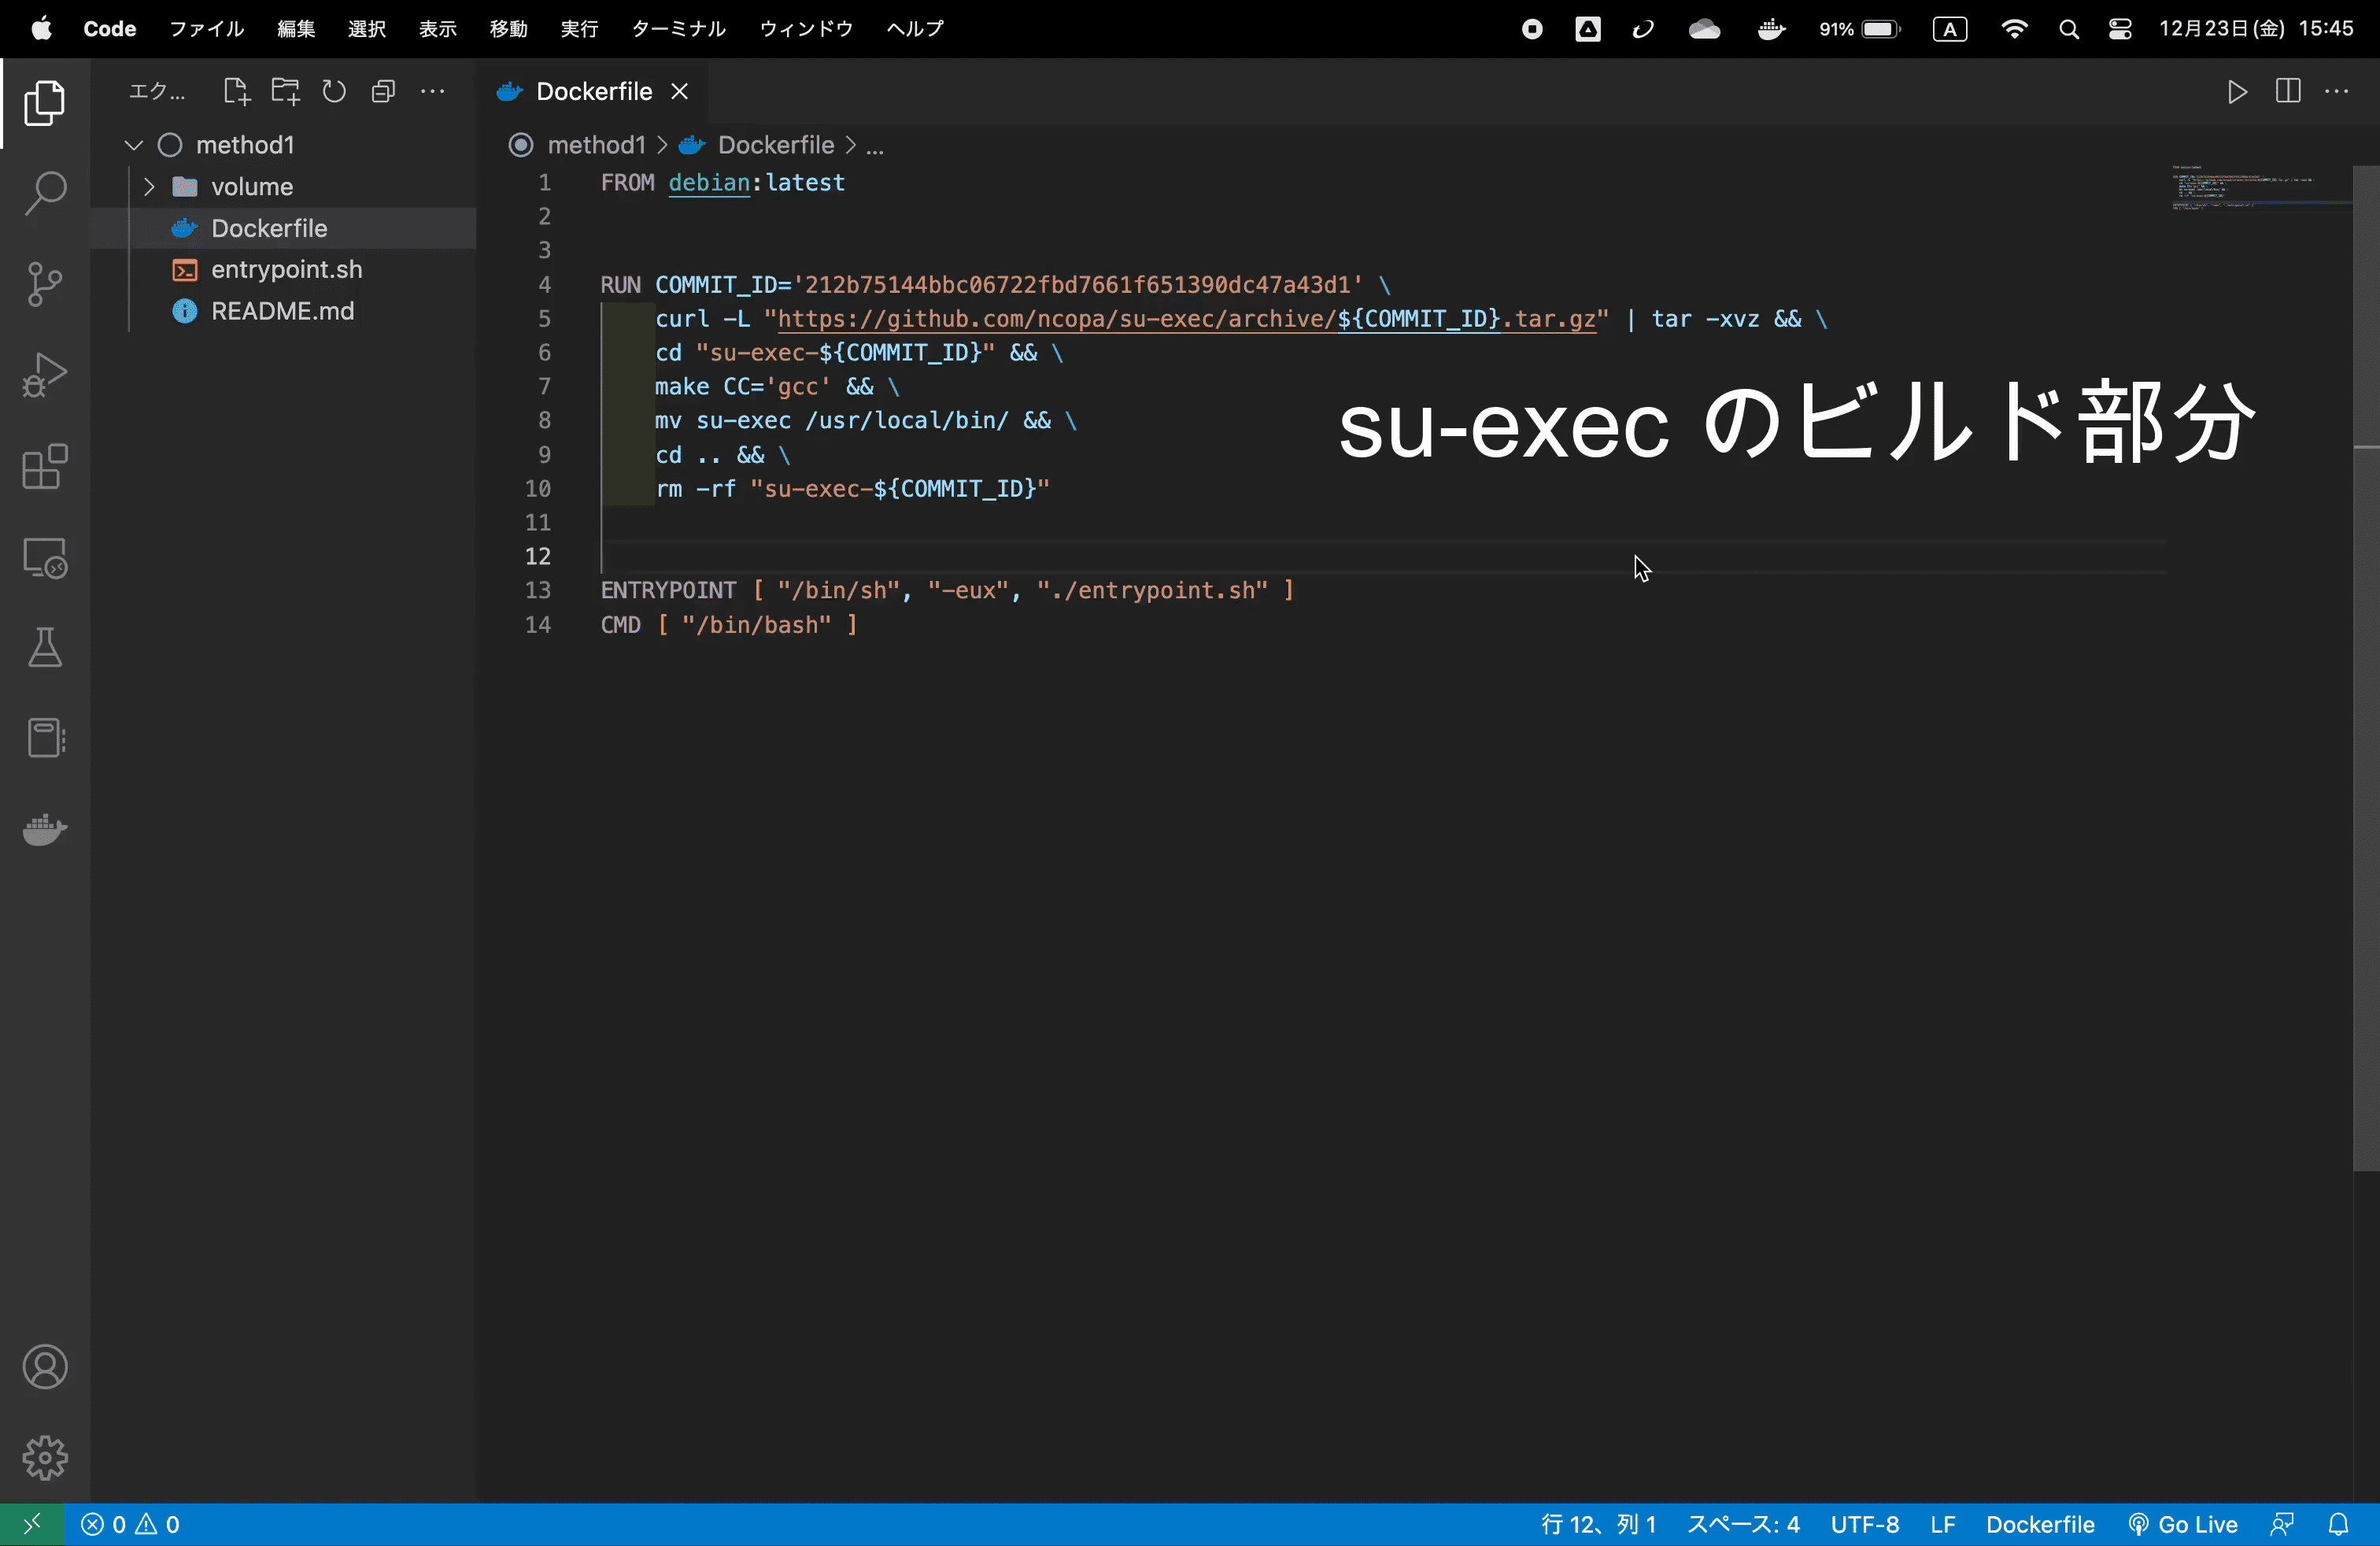
\includegraphics[keepaspectratio, width=\linewidth]{img/thumbnail1.png}
}

    \pause
    \begin{tikzpicture}[remember picture]
        \useasboundingbox (0.0, 0.0);
        \begin{scope}[shift={(current page.south west)}]
            \node[probrem] at (6.4, 4.0) {気にかけることが多い};
        \end{scope}
    \end{tikzpicture}
\end{frame}


\begin{frame}{開発途中のDockerfileから逐一生成するコンテナで\\動作確認をしながら,Dockerfileを開発する例}

\href{https://user-images.githubusercontent.com/103095414/209308620-3ed140c5-6c34-4dba-925d-e29227639d16.mp4}{
    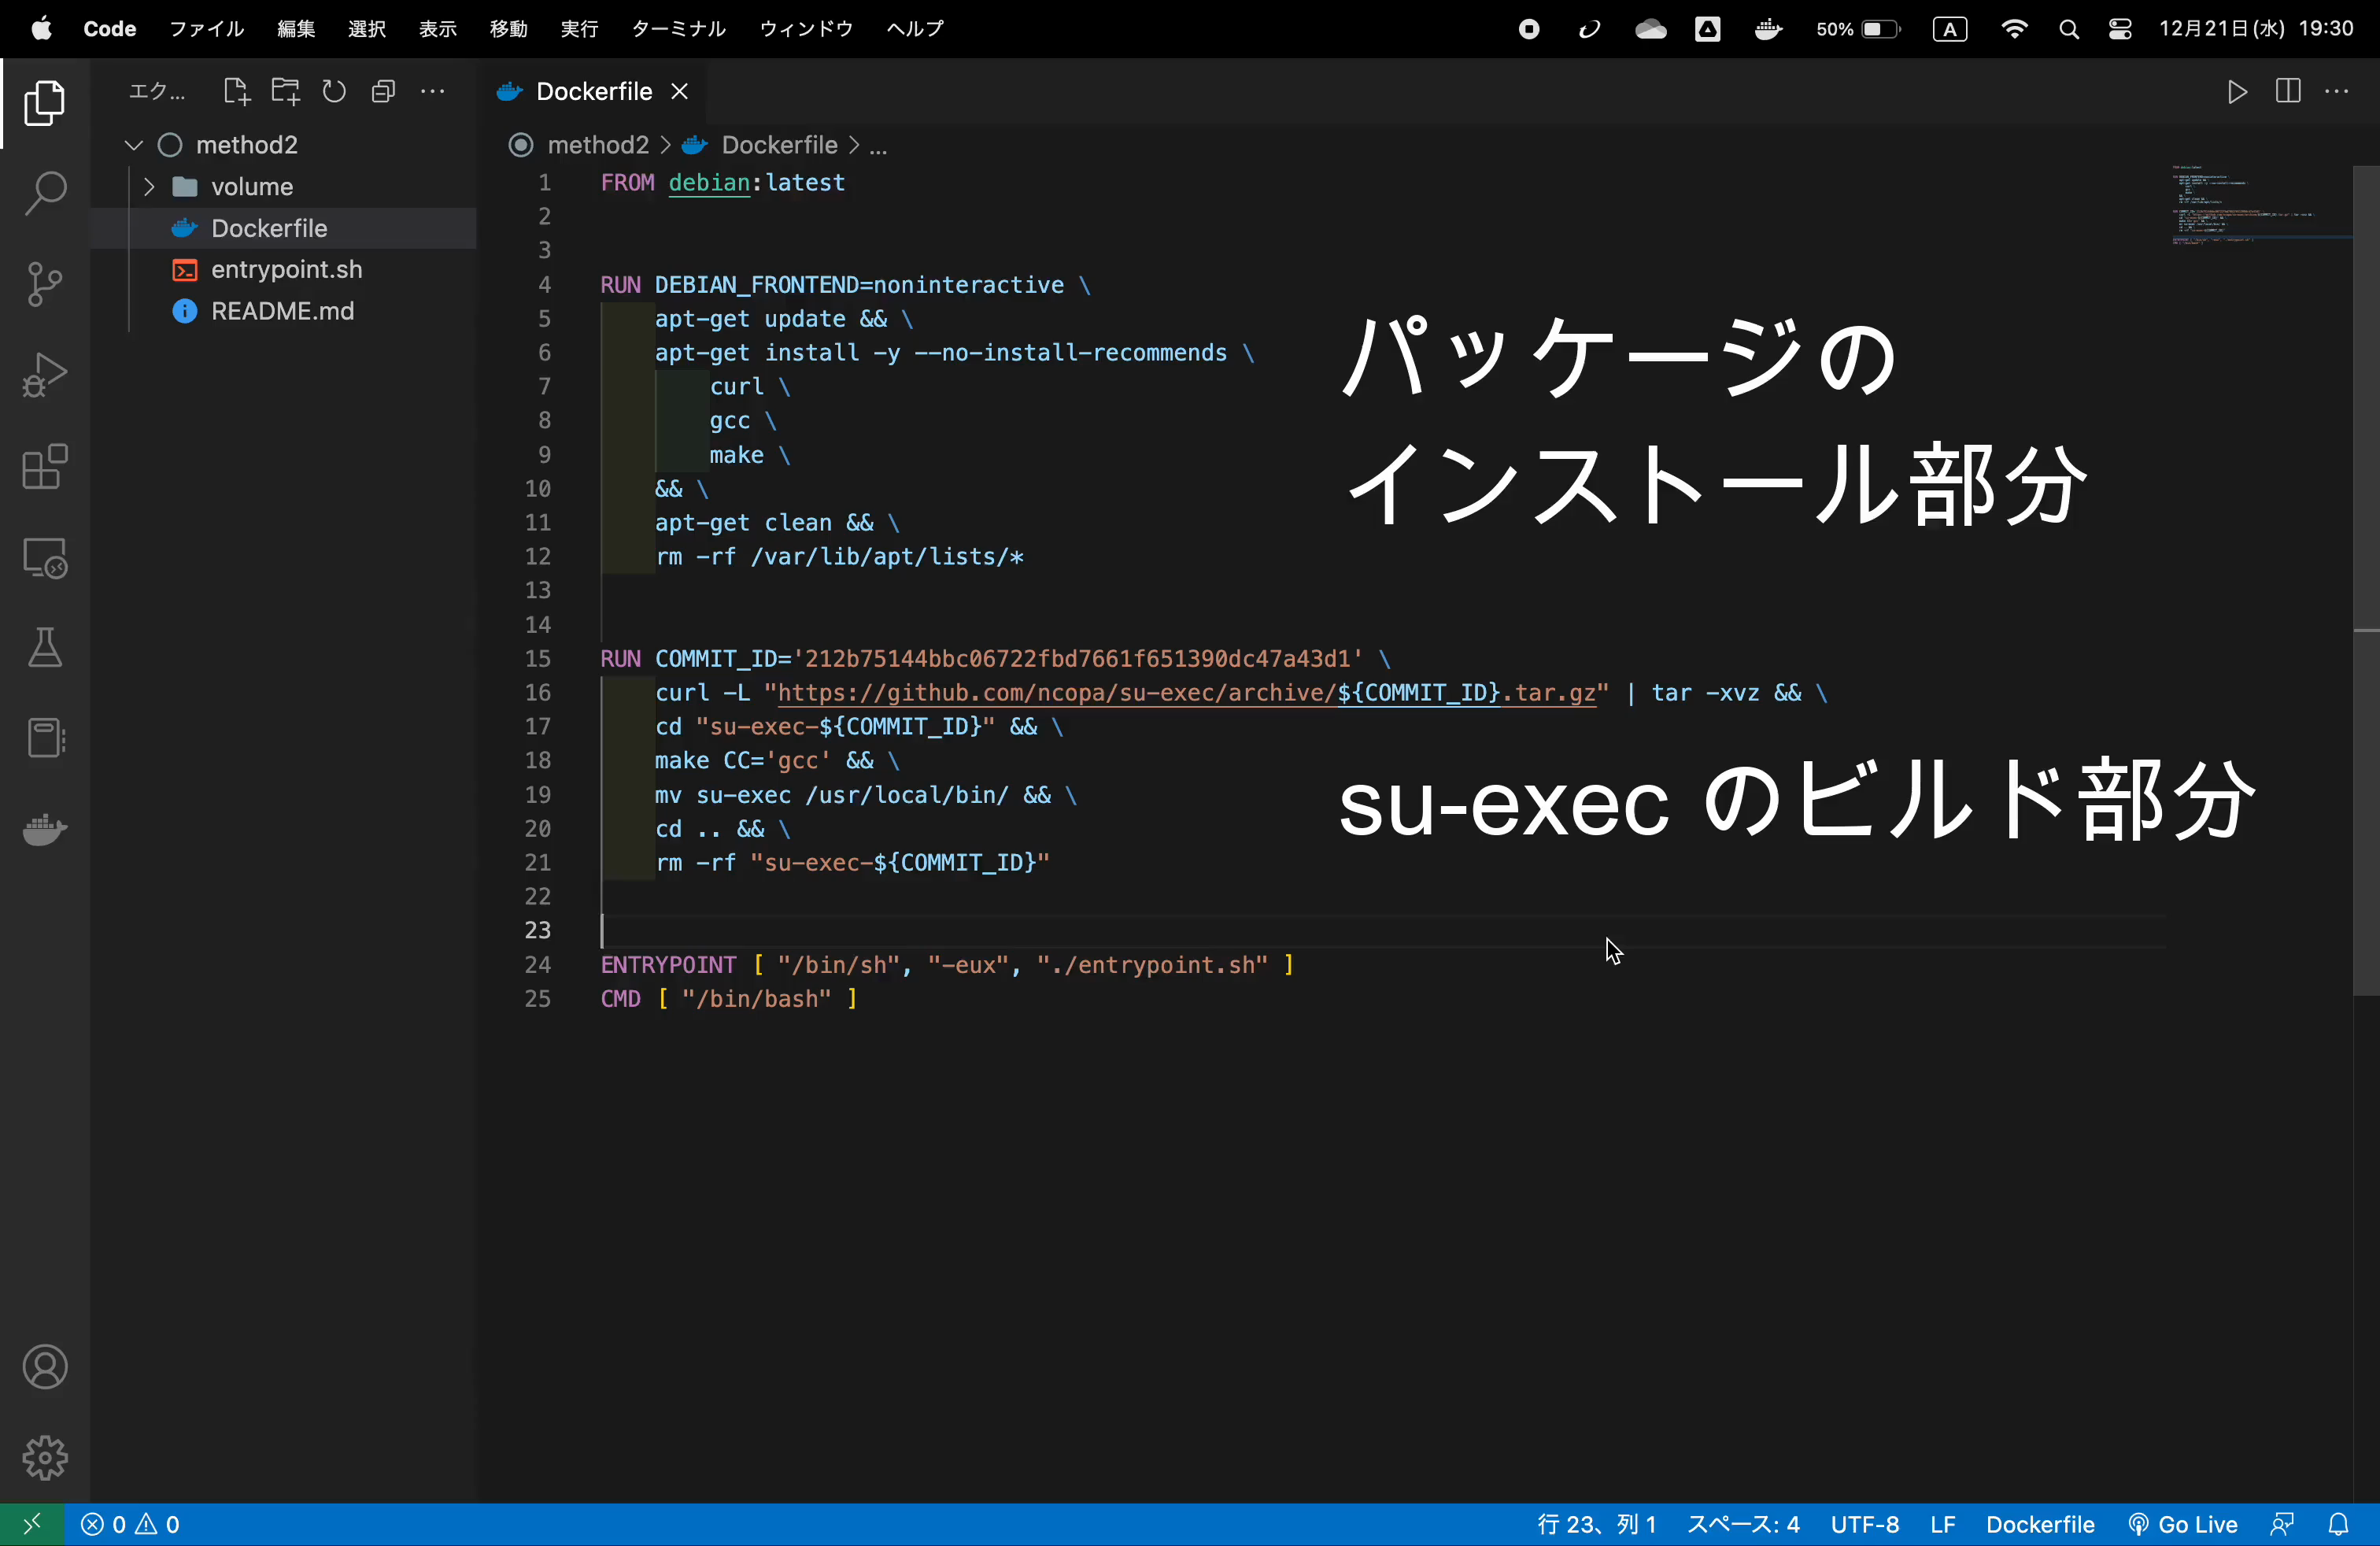
\includegraphics[keepaspectratio, width=\linewidth]{img/thumbnail2.png}
}

    \pause
    \begin{tikzpicture}[remember picture]
        \useasboundingbox (0.0, 0.0);
        \begin{scope}[shift={(current page.south west)}]
            \node[probrem] at (6.4, 4.0) {時間ロスが大きい};
        \end{scope}
    \end{tikzpicture}
\end{frame}


\begin{frame}{本ツールを用いて,Dockerfileを開発する例}
    % TODO: 開発動画
    
\end{frame}


\begin{frame}{本ツールの特長}
    Dockerfileの効率的な開発手法が必要.
    \vskip0.5zh

    \hskip3.0zw
    {\huge $\Downarrow$}
    \vskip0.5zh

    \textcolor{blue!75}{インタラクティブツールとしての側面}

    ユーザがコンテナ内で動作確認をしながら環境構築するだけで,
    \textcolor{red!75}{自動的に}Dockerfileを生成してくれる.
\end{frame}


\begin{frame}{これだけでは優れたDockerfileにはならない}
    前述の方法で自動生成したDockerfile

    % TODO: リファクタリング・最適化前の画像
    

    \begin{tikzpicture}[remember picture]
        \useasboundingbox (0.0, 0.0);
        \begin{scope}[shift={(current page.south west)}]
            \only<2>{\node[probrem] at (6.4, 4.0) {見づらい};}

            \begin{onlyenv}<3>
                \node[callout, callout absolute pointer={(5.6, 2.2)}] at (8.8, 3.8) {絶対パス指定の方がいい};
                \node[callout, callout absolute pointer={(5.6, 1.2)}] at (8.8, 1.8) {集約した方がいい};
            \end{onlyenv}
        \end{scope}
    \end{tikzpicture}
\end{frame}


\begin{frame}{Dockerfileのリファクタリング・最適化を行ってみる}
    リファクタリング・最適化後のDockerfile

    % TODO: リファクタリング・最適化後の画像
    
\end{frame}


\begin{frame}{本ツールの特長}
    \textcolor{blue!75}{インタラクティブツールとしての側面}

    ユーザがコンテナ内で動作確認をしながら環境構築するだけで,
    \textcolor{red!75}{自動的に}Dockerfileを生成してくれる.

    \vskip1.0zh
    \textcolor{blue!75}{リファクタリングツールとしての側面}

    上のようにして生成したDockerfileに,ベストプラクティスに基づいたリファクタリング・最適化を行うことができる.
\end{frame}




\section{簡単な使い方}

\begin{frame}[fragile]{手順 1/5\\「本ツールのリポジトリをクローンする」}
    本ツールの\href{https://github.com/posl/inada_docker_interactive}{GitHubページ}のmainブランチをクローンする.
    \vskip2.0zh

    実行例
\begin{lstlisting}[]
URL=https://github.com/posl/inada_docker_interactive
git clone --depth 1 "${URL}"
\end{lstlisting}

\end{frame}


\begin{frame}[fragile]{手順 2/5\\「開発用のディレクトリを用意する」}
    開発中のDockerfileが入るディレクトリを用意する.

    \textcolor{red!75}{コンテナ内にコピーしたいファイル}もここに入れる.
    \vskip2.0zh

    実行例
\begin{lstlisting}[]
cd ./inada_docker_interactive
mkdir app
\end{lstlisting}

\end{frame}


\begin{frame}[fragile]{手順 3/5\\「開発用のコンテナを起動し,開発を開始する」}
    開発用のディレクトリを設定しながら,\textcolor{red!75}{exec.sh}を実行する.

    実行後は,指定したベースイメージに\textcolor{red!75}{bash}で入った状態.
    \vskip2.0zh

    実行例
\begin{lstlisting}[]
sh exec.sh -d ./app -n debian
\end{lstlisting}

\end{frame}


\begin{frame}{手順 4/5\\「動作確認をしながら,お好みの環境構築を行う」}
    コンテナ内で動作確認をしながら,環境構築するだけで,

    それと同時進行で,\textcolor{red!75}{自動的に}Dockerfileが作られていく.
    \vskip2.0zh

    ただし,次の場合は本ツールの機能を使うこと.
    \begin{itemize}
        \item パッケージのインストール $\longrightarrow$ dit package
        \item ホスト環境からのファイルのコピー $\longrightarrow$ dit copy
    \end{itemize}
\end{frame}


\begin{frame}[fragile]{手順 5/5\\「Dockerfileのリファクタリング・最適化を行う」}
    最後に,Dockerfileのリファクタリング・最適化を行う.
\begin{lstlisting}[]
dit optimize
\end{lstlisting}

    \vskip2.0zh
    Dockerfileが完成したので,開発を終了する.
\begin{lstlisting}[]
exit
\end{lstlisting}
\end{frame}




\section{まとめ}

\begin{frame}{今後の展望}
    \begin{itemize}
        \setlength{\itemsep}{1.0zh}
        \item 実装途中の部分を完成させる.
        \item ドキュメントページを作成する.
        \item Dockerfileに命令を追加する機能を充実させる.
        \item マルチステージビルドに対応する.
        \item 標準入力を捕捉できるようにする.
    \end{itemize}
\end{frame}


\begin{frame}{まとめ}
    背景
    \begin{itemize}
        \setlength{\itemsep}{0.8zh}
        \item Dockerfileを効率的に開発するためのツールがない.
        \item Dockerfileのリファクタリング・最適化ツールがない.
    \end{itemize}

    \vskip2.0zh
    提案ツール
    \begin{itemize}
        \setlength{\itemsep}{0.8zh}
        \item コンテナ内のbash環境で,対話的に作業する.
        \item 動作確認だけに集中して,Dockerfileが作成できる.
        \item リファクタリング・最適化後のDockerfileが得られる.
    \end{itemize}
\end{frame}




% ページ番号を合わせる
\section{参考資料(p.33〜)}

\begin{frame}{基本情報}
    \begin{itemize}
        \setlength{\itemsep}{0.8zh}
        \item ツールのDockerfileから開発用のコンテナを起動し,bashコマンドを用いて,対話的に作業する.
        \item 開発用のディレクトリには,以下などが入る.
        \begin{itemize}
            \item Dockerfile(下書き・完成版)
            \item 履歴ファイル
            \item ユーザがコンテナ内にコピーしたいファイル
        \end{itemize}
        \item ツールの機能の利用は,dit\footnotemark[1]コマンドから行う.
        \item /dit\footnotemark[1]ディレクトリにツールが利用するファイルが入るが,不用意にそれらに触れてはいけない.
    \end{itemize}

    \footnotetext[1]{Docker Interactive Toolの略.}
\end{frame}


\newcommand{\MyFunctionTable}[4]{
    \begin{frame}{機能要件}
        \begin{enumerate}
            \setbeamercovered{dynamic}
            \setlength{\itemsep}{0.8zh}
            \item<#1> シェルで任意のコマンドを実行するたびに,その必要性を判断して,対応する命令をDockerfileに追加する機能.
            \item<#2> CUI上でDockerfileを編集する機能.
            \item<#3> ベストプラクティスに基づいて,作成されたDockerfileのリファクタリング・最適化を行う機能.
            \item<#4> Dockerfileの開発を任意のタイミングで中断・再開できるようにする機能.
        \end{enumerate}
    \end{frame}
}

\MyFunctionTable{1}{1}{1}{1}
\MyFunctionTable{1}{0}{0}{0}


\begin{frame}[fragile]{機能1\\「シェルで任意のコマンドを実行するたびに処理を行う」}
    bashのシェル変数PROMPT\_COMMANDを使用する.
    \vskip2.0zh

    使用例
\begin{lstlisting}[language=sh]
# records the latest exit status
PROMPT_COMMAND='echo "$?" > /tmp/exit-status'
\end{lstlisting}

\end{frame}


\begin{frame}{機能1\\「コマンドの反映の要否を判断する」}
    以下の設定情報(詳細は後述)
    \begin{itemize}
        \setlength{\itemsep}{0.8zh}
        \item 5つの反映モード
        \item 反映しないコマンドと条件をまとめたJSONファイル(以下「\textcolor{red!75}{ignoreファイル}」と称する)
    \end{itemize}
    とコマンドラインの解析結果などを元に判断する.

    \vskip2.0zh
    設定情報はそれぞれ,`\textcolor{blue!75}{dit config}'・`\textcolor{blue!75}{dit ignore}'で編集できる.
\end{frame}


\begin{frame}{機能1\\「対応する命令をDockerfileに追加する」}
    以下のような変換規則
    \begin{itemize}
        \item 代入文 $\longrightarrow$ ARG命令
        \item cdコマンド $\longrightarrow$ WORKDIR命令
    \end{itemize}

    以下のような反映ルール
    \begin{itemize}
        \item 通常ファイルへのリダイレクトを行う部分は反映する.
        \item パイプラインの切り詰めは右からのみ行う.
    \end{itemize}
    を適用して,追加処理を行う.

    \vskip1.0zh
    このような変換処理は,`\textcolor{blue!75}{dit convert}'が担当する.
\end{frame}


\begin{frame}{機能1 設定情報(config)}
    5つの反映モード
    \begin{description}
        \item[no-reflect] Dockerfileに命令を追加しない.
        \item[strict] できる限り,ignoreファイルの設定に従う.
        \item[normal] 処理のまとまりを考え,反映の要否を変更する.
        \item[simple] 単純なコマンド以外はそのまま反映する.
        \item[no-ignore] 実行されたコマンドラインは必ず反映する.
    \end{description}

    \vskip1.0zh
    \textcolor{red!75}{strictとnormalの違い}

    `hoge \&\& piyo'が実行された場合,
    \begin{description}
        \item[strict] hogeだけを反映する可能性がある
        \item[normal] ひとまとめに,反映の要否を決定する
    \end{description}
\end{frame}


\begin{frame}[fragile]{機能1 設定情報(ignore)}
    ignoreファイルの例
\begin{lstlisting}[language=json]
{
    "ls": null,
    "dir": "ls",
    "wget": {
        "short_opts": "O:",
        "long_opts": {
            "output-document": 1
        },
        "optargs": {
            "output-document": "O",
            "O": [
                "-"
            ]
        },
        "detect_anymatch": true
    }
}
\end{lstlisting}

\end{frame}


\begin{frame}{機能1 変換処理の流れ(convert)}
    \begin{tikzpicture}[remember picture]
        \useasboundingbox (0.0, 0.0);
        \begin{scope}[shift={(current page.south west)}]
            \node[progress20] (p1) at (6.8, 7.6) {直前の終了ステータスを判定};
            \node[progress20] (p2) at (6.8, 6.4) {現在の反映モードを判定};
            \node[progress20] (p3) at (6.8, 5.2) {コマンドラインを解析・展開};
            \node[progress10] (p4) at (2.2, 4.0) {変換規則の適用};
            \node[progress20] (p5) at (6.8, 2.8) {ignoreファイル・反映ルールの適用};

            \node[success] (g1) at (2.2, 1.0) {対応する命令を追加};
            \node[success] (g2) at (6.8, 1.0) {RUN命令を追加};
            \node[failure] (g3) at (11.4, 1.0) {失敗で終了};

            \coordinate (c1) at (2.2, 2.8);
            \coordinate (c2) at (6.8, 4.0);
            \coordinate (c3) at (11.4, 2.8);
            \coordinate (c4) at (11.4, 6.4);
            \coordinate (c5) at (11.4, 7.6);

            \foreach \u / \v in {p1/p2,p2/p3,p3/p5,p4/g1,p5/g2,c1/p5,c2/p4}
                \draw[arrows = {-Stealth}] (\u) -- (\v);

            \foreach \u / \v in {p1/c5,p2/c4,p5/c3,c5/g3}
                \draw[red, arrows = {-Stealth}] (\u) -- (\v);

            \begin{tikzpicture}[remember picture, overlay]
                \only<2>{\node[callout, callout absolute pointer={(p2.north)}] at (1.2, 3.0) {成功ならば};}
                \only<3>{\node[callout, callout absolute pointer={(p3.north)}] at (1.2, 1.8) {no-reflect以外};}
                \only<4>{\node[callout, callout absolute pointer={(p4.east)}] at (1.2, 1.0) {候補にだけ};}
                \only<5>{\node[callout, callout absolute pointer={(c3)}] at (7.2, 0.0) {反映するものがなければ};}
            \end{tikzpicture}
        \end{scope}
    \end{tikzpicture}
\end{frame}


\begin{frame}[fragile]{機能1 変換処理の具体例(convert)}
    以下の設定で,次のコマンドラインの実行が成功した場合.
    \vskip1.0zh

    設定情報
    \begin{description}[labelwidth=10zw]
        \item[反映モード] strict
        \item[ignoreファイル] 先述の内容
    \end{description}

    \vskip1.0zh
    コマンドライン
\begin{lstlisting}[language=sh]
# URL=https://ftp.gnu.org/gnu/bash/bash-5.1.16.tar.gz
wget -O - "${URL}" | tar -xvz && dir -AFl bash-5.1.16
\end{lstlisting}

\end{frame}


\begin{frame}{機能1 変換処理の具体例(convert)}
    コマンドラインの解析・展開後
    \xytree[3]{
        & & \xynode[-1,1]{`\&\&'}  \\
        & \xynode[-1,1]{`$|$'} & & \xynode{`dir -AFl bash-5.1.16'}  \\
        \xynode{`wget -O - "\$\{URL\}"'} & & \xynode{`tar -xvz'}
    }

    \vskip0.5zh
    \begin{table}[hbtp]
        \centering
        \begin{tabular}{lccc}
            \hline
            適用 & `wget' & `tar' & `dir' \\
            \hline \hline
            ignoreファイル \onslide<2->{& 反映しない & 反映する & 反映しない} \\
            反映ルール \onslide<3->{& \textcolor{red!75}{反映する} & 反映する & 反映しない} \\
            \hline
        \end{tabular}
    \end{table}

    \onslide<4>{よって,`RUN wget -O - "\$\{URL\}" $|$ tar -xvz'を追加する.}
\end{frame}


\MyFunctionTable{0}{1}{0}{0}


\begin{frame}{機能2\\「ホスト環境からファイルをコピーする」}
    \textcolor{blue!75}{dit copy}

    \hskip1.0zw
    ホスト環境からコンテナ内へのファイルのコピーを行い,その内容をCOPY・ADD命令としてDockerfileに反映する.
    \vskip2.0zh

    このコマンドを使うと,
    \begin{itemize}
        \item COPY命令とcpコマンドの仕様の違いを意識せず済む.
        \item ADD命令のtar展開機能を利用できる.
    \end{itemize}
\end{frame}


\begin{frame}{機能2\\「パッケージをインストールする」}
    \textcolor{blue!75}{dit package}

    \hskip1.0zw
    最適化された形式で,パッケージのインストールを行い,その内容をRUN命令としてDockerfileに反映する.
    \vskip2.0zh

    このコマンドを使うと,
    \begin{itemize}
        \item イメージサイズの削減に効果的な方法で実行される.
        \item パッケージマネージャの違いをあまり意識せず済む.
    \end{itemize}
\end{frame}


\begin{frame}[fragile]{機能2\\「Dockerfileに命令を追加する」}
    \textcolor{blue!75}{dit reflect}

    \hskip1.0zw
    各種ログを取りながら,Dockerfileに命令を追加する.
    \vskip1.0zh
    実行例

\begin{lstlisting}[language=sh]
# reflects the contents of `./instr.txt' in Dockerfile
dit reflect -d instr.txt
\end{lstlisting}

\begin{lstlisting}[language=sh]
# reflects the input contents as they are in Dockerfile
dit reflect -dp -
\end{lstlisting}

\end{frame}


\begin{frame}[fragile]{機能2\\「Dockerfileから指定した行を削除する」}
    \textcolor{blue!75}{dit erase}

    \hskip1.0zw
    条件にマッチする行を,Dockerfileから削除する.
    \vskip1.0zh
    実行例

\begin{lstlisting}[language=sh]
# deletes the lines added just before from Dockerfile
dit erase -d
\end{lstlisting}

\begin{lstlisting}[language=sh]
# deletes all LABEL instructions from Dockerfile
dit erase -diy -E '^LABEL[[:space:]]'
\end{lstlisting}

\end{frame}


\MyFunctionTable{0}{0}{1}{0}


\begin{frame}{機能3\\「Dockerfileのリファクタリング・最適化を行う」}
    \textcolor{blue!75}{dit optimize}

    \hskip1.0zw
    下書きのDockerfileから,完成版のDockerfileを生成する.
    \vskip1.0zh

    処理内容の例
    \begin{itemize}
        \item WORKDIR命令のオペランドを絶対パスにする.
        \item ENV・ARG命令の重複や無意味な再定義を取り除く.
        \item 連続するRUN命令をまとめる.
        \item 可読性を向上させるための整形を行う.
    \end{itemize}
\end{frame}


\MyFunctionTable{0}{0}{0}{1}


\begin{frame}{機能4\\「Dockerfileの開発を中断・再開する」}
    履歴ファイルというものを導入することで実現する.

    \vskip1.0zh
    \begin{description}
        \setlength{\itemsep}{1.0zh}
        \setlength{\leftskip}{-1.0zw}
        \item[開発中] 履歴ファイル用の反映モードとignoreファイルを別で用意し,Dockerfileと同じようにして編集する.
        \item[再開時] sourceコマンド・historyコマンドで履歴ファイルを読み込み,環境を再現する.
    \end{description}
\end{frame}


\end{document}